%------------------------------------------------
% Quick reference. 
%------------------------------------------------
%
% Для вставки картинок:
%
%--------         Комманда
%
%\begin{figure}[H]
%	\includegraphics{img_name}
%	\caption{some caption}
%	\label{some_pic}
%\end{figure}
%
%--------        Переменные
%
% img_name     <- Название картинки в папке img.
% some_caption <- подпись картинки.
% label        <- лейбл нужен для ссылок на картинку.
% H            <- расположение картинки на странице.
%
%--------         Пример
%
%\begin{figure}[H]
%	\includegraphics{pic1.jpg}
%	\caption{График}
%	\label{grapics1}
%\end{figure}
%
%------------------------------------------------
%
% Для референса по лейблу:
%
%--------         Комманда
%
% Для ссылки используется \eqref{ref}.
%
%--------        Переменные
%
% ref          <- указанный лейбл в директиве \label{ref}
%                 Ссылку можно сделать на любой объект имеющий \label{•}
%
%--------         Пример
%
% \eqref{graphics1}
%
%------------------------------------------------
%
% Для листинга кода:
%
%--------         Комманда
%
% \lstinputlisting[language=lang,mathescape=true]{src}
%--------        Переменные
%
% lang         <- язык на котором написан исходный код, например "python" или "C++".
% mathescape   <- если в исходниках есть формулы LaTeX, то они будут представлены как формулы.
% src          <- путь до файла исходников.
%
%--------         Пример
%
% \lstinputlisting[language=C++,mathescape=false]{./src/main.cpp}
%
%------------------------------------------------
%
% Для вставки таблиц:
%
%--------
%\begin{table}[H]
%	\centering
%	\caption{ capt }
%	\begin{tabularx}{0.9\textwidth}{ | Y | Y | }
%		\hline
%		lines
%	\end{tabularx}
%	\label{tab1}
%\end{table}
%--------
% caption      <- Подпись таблицы.
% tab1         <- лейбл нужный для ссылки на таблицу.
% | Y | Y |    <- количество и формат столбцов.
% Y            <- Тип столбца.
%                 В данном случае определены кастомные столбцы Y (Спасибо Максиму Наумову)
% |            <- обозначает границы столбца.
%                 То есть, если будет указано |Y Y|, то столбцы внутри строк разделены не будут.
% H            <- То же самое, что и у картинок.
% lines        <- непосредственно элементы таблицы.
%                 Разделяются знаком "&", оканчивать каждую строку лучше \\ \hline
%
%--------         Пример
%\begin{table}[H]
%	\centering
%	\caption{ capt }
%	\begin{tabularx}{0.9\textwidth}{ | Y | Y | }
%		\hline
%		str1 & str2 \\ \hline
%		str1 & str2 \\ \hline
%		str1 & str2 \\ \hline
%		str1 & str2 \\ \hline
%		str1 & str2 \\ \hline
%	\end{tabularx}
%	\label{tab1}
%\end{table}
%------------------------------------------------

\documentclass[12pt, fleqn, a4paper]{extarticle}

\makeatletter
\renewcommand*\l@section{\@dottedtocline{1}{1.5em}{2.3em}}



%\includegraphics{universe}

\usepackage[utf8]{inputenc}
\usepackage[T2A]{fontenc}
\usepackage[russian]{babel} % указывает язык документа
\usepackage[left=3cm,right=2cm,top=2cm,bottom=2cm,bindingoffset=0cm]{geometry}
\usepackage{lastpage}
\usepackage{fancyhdr}
\usepackage{titlesec}
\usepackage{graphicx} % для вставки картинок
\usepackage[intlimits]{mathtools} % математические дополнения
\usepackage{amssymb}
\usepackage[tableposition=top]{caption}
\usepackage{subcaption}
\usepackage{indentfirst}
\usepackage{minted}
\usepackage{tabularx}
\usepackage{tabulary}
\usepackage{multirow}
\usepackage{float}
\usepackage[figure,table]{totalcount}
\usepackage{diagbox}
\usepackage[german=guillemets]{csquotes}
\usepackage{fontspec} 
\usepackage{enumitem}
%\usepackage{mathptmx}% http://ctan.org/pkg/mathptmx
%\usepackage{showframe}
\usepackage{hyperref}

\setlength{\parindent}{1.2cm}

\setlength{\mathindent}{1.2cm}

\defaultfontfeatures{Ligatures={TeX},Renderer=Basic} 
\setmainfont[Ligatures={TeX,Historic}]{Times New Roman}

%\setlist[enumerate]{itemindent=\dimexpr\labelwidth+\labelsep\relax,leftmargin=0pt}

%\setlength{\section*}{0.5cm}
%\usepackage{minted}
%\usepackage{fancyvrb}
%\usepackage{newtxtext}

%\titleformat{\section}[hang]{\bfseries\LARGE\centering}{}{1em}{}

%\setlist[enumerate]{itemindent=\dimexpr\labelwidth+\labelsep\relax,leftmargin=0pt}
\setlist[enumerate,itemize]{leftmargin=1.3cm,itemindent=0.4cm}

\titleformat{\section}{\large\bfseries\centering}{\thesection}{0.5em}{\MakeUppercase}
\titleformat{\subsection}[block]{\bfseries\hspace{1em}}{\thesubsection}{0.5em}{}
%\setlength{\subsection*}{1.5cm}
%\setlength{\parindent}{4em}

%\setlength{\parindent}{1.5cm}

\captionsetup[figure]{labelfont={it},textfont={it},name={Рисунок},labelsep=endash, skip=5pt}
\captionsetup[table]{labelfont={it},textfont={it},name={Таблица},labelsep=endash,singlelinecheck=false, skip=5pt, margin=1cm}


%\renewcommand{\baselinestretch}{1.5}
\linespread{1.5} % полуторный интервал
\frenchspacing
\graphicspath{ {images/} }

  %-------------------------------------------
  % Переменные
  %-------------------------------------------

  \newcommand{\firstAuthorSurName}{Наумов} 					                           % Фамилия автора.
  \newcommand{\firstAuthorInitials}{ М. Е.} 					                           % Фамилия автора.
  % \newcommand{\leftcolon}{Уравнения Математической Физики}
  %\newcommand{\secondAuthorSurName}{Родин} 					                           % Фамилия автора.
 % \newcommand{\secondAuthorInitials}{ И. А.} 					                           % Фамилия автора.
  \newcommand{\teacherName}{Кириленко М.С.}				                               % Имя преподавателя.
%  \newcommand{\variantNumber}{25} 							                           % Номер варианта.
  \newcommand{\groupNumber}{6409-010302D} 				                               % Номер группы.
  %\newcommand{\subjectTitle}{Отчет по лабораторной работе No1}                                  % Название предмета.
%  \newcommand{\taskTitle}{Дисциплина \enquote{Уравнения математической физики}} 		  % Название работы.
%  \newcommand{\theme}{АНАЛИТИЧЕСКОЕ РЕШЕНИЕ КРАЕВЫХ ЗАДАЧ МАТЕМАТИЧЕСКОЙ ФИЗИКИ} 		  % Название работы.
  
  %-------------------------------------------
  % Ссылки в оглавлении
  %-------------------------------------------
  

\hypersetup{
    colorlinks,
    citecolor=black,
    filecolor=black,
    linkcolor=black,
    urlcolor=black
}

  %-------------------------------------------
  % Стиль футеров и хедеров
  %-------------------------------------------

\pagestyle{fancy}
\fancyhead[L, R]{}
\fancyfoot[L]{}
\fancyfoot[R]{}
\renewcommand{\footrulewidth}{0pt}
\renewcommand{\headrulewidth}{0pt}

%\renewcommand\subsectionfont{\normalfont\normalsize\bfseries}

\def\l@subsection{\@dottedtocline{2}{3.8em}{3.2em}}

\newcolumntype{Y}{>{\centering\arraybackslash}X}

\begin{document}

%----------------------------------------------------------------------------------------
%	TITLE PAGE
%----------------------------------------------------------------------------------------
\pagenumbering{Alph}

\begin{titlepage}
							
	\center
							
	%------------------------------------------------
	%	Заголовки
	%------------------------------------------------
							
	\textsc{Министерство образования и науки Российской Федерации}\\[-0.15cm]
	\textsc{Федеральное государственное автономное образовательное учреждение \\[-0.15cm] высшего образования}\\[-0.15cm] 
	\textsc{«Самарский национальный исследовательский университет \\[-0.15cm] имени академика С.П.Королёва»}\\[0.5cm]
	\textsc{Институт информатики, математики и электроники}\\[-0.7em]
	\textsc{Факультет информатики}\\[-0.7em]
	\textsc{Кафедра технической кибернетики}\\[-1em]
						
	%------------------------------------------------
	%	Название работы
	%------------------------------------------------
							
	\vfill\vfill
						    
							
	{\textbf{Отчет по лабораторной работе No2}}\\[-0.7em]
	{\textbf{по курсу «Оптоинформационные технологии и системы»}}\\
	{\textbf{Вариант 6}}\\
	
    \vfill\vfill\vfill\vfill\vfill\vfill\vfill\vfill\vfill
							
	\begin{minipage}{1\textwidth}
		\begin{center}
			\begin{tabularx}{\textwidth}{X l}
				Выполнил студент:        & \firstAuthorSurName \firstAuthorInitials \\
				Группа:                    & 6409                     		           \\
				Преподаватель:                  & \teacherName         		                \\
			\end{tabularx}
		\end{center}
	\end{minipage}
							
						
	%------------------------------------------------
	%	Дата
	%------------------------------------------------
							
	\vfill\vfill\vfill
					
	{\centering Самара \the\year}
							
							
\end{titlepage}

\pagenumbering{arabic}

\setcounter{page}{2}


%------------------------------------------------
%Задание
%------------------------------------------------

\section*{Задание}
{
	\begin{enumerate}
	    \item Реализовать одномерное финитное преобразование Фурье с помощью
применения алгоритма БПФ.

	\item Построить график гауссова пучка $\mathrm{e}^{-x^2}$. Здесь и далее для каждого графика следует строить отдельно графики амплитуды и фазы. Амплитуда находится как модуль каждого значения функции, фаза -- как аргумент (или с помощью функции atan2).

	\item Убедиться в правильности реализации преобразования, подав на вход гауссов пучок $\mathrm{e}^{-x^2}$ -- собственную функцию преобразования Фурье. На выходе тоже должен получиться гауссов пучок (построить график на правильной области определения $[-\tilde{b}, \tilde{b}]$). Рекомендуемая входная область: $[−a, a]$ = $[−5, 5]$.

	\item Реализовать финитное преобразование Фурье стандартным методом численного интегрирования (например, методом прямоугольников). Важно: необходимо вычислить интеграл для каждого дискретного значения $u$, чтобы получить результат в виде вектора. На вход преобразования вновь следует подавать гауссов пучок.

	\item Построить результаты двух разных реализаций преобразования на одном изображении (одно для амплитуды, одно для фазы) и убедиться, что они совпадают.
	
	\item Используя первую реализацию преобразования, подать на вход световое поле, отличное от гауссова пучка, в соответствии со своим вариантом. Построить графики самого пучка и результата преобразования.
	
	\item Рассчитать аналитически результат преобразования своего варианта поля и построить график на одной системе координат с результатом, полученным в предыдущем пункте.
	\end{enumerate}
}
\newpage

\section*{Алгоритм реализации оптического финитного преобразования Фурье через использование БПФ}
{
	\begin{enumerate}
		\item Провести дискретизацию входной функции $f(x)$ в вектор $f$ с размерностью N.
		\item Дополнить вектор $f$ и слева, и справа необходимым числом нулей до размерности $M$.
		\item Разбить вектор f на две половины и поменять их местами.
		\item Выполнить БПФ от $f$ и умножить результат на шаг $h_x$ , получив вектор $F$.
		\item Разбить вектор $F$ на две половины и поменять их местами.
		\item \enquote{Вырезать} центральную часть вектора $F$, оставив $N$ элементов.
	\end{enumerate}
}
\newpage

%------------------------------------------------
% Начало основной части
%------------------------------------------------
\titleformat{\section}{\large\bfseries}{\thesection}{0.5em}{}
\titlespacing*{\section}{\parindent}{1ex}{1em}
\section*{Выполнение задания}
{
	\begin{enumerate}
		\item {
			Одномерное финитное преобразование Фурье записывается в виде \eqref{fin_transform};
			\begin{equation}\label{fin_transform}
			F_a(u) = \Phi_a \left[ f(x) \right] (u) = \int\limits_{-a}^{a} f(x) e^{-2 \pi i x u} \,dx,
			\end{equation}
			где $f(x)$ -- финитная функция, $F_a(u)$ -- спектр, $\Phi_a$ -- оператор финитного преобразования Фурье.
			
			Приведём реализацию одномерного финитного преобразования Фурье (полный код представлен в приложении А):
			
		\inputminted[breaklines, mathescape, fontsize=\footnotesize]{octave}{./src/solve_with_fft.m}
		}
		
		\item {
			На рисунке \ref{gauss} изображены: график гауссова пучка, графики амплитуды и фазы.
			
			\begin{figure}[H]
				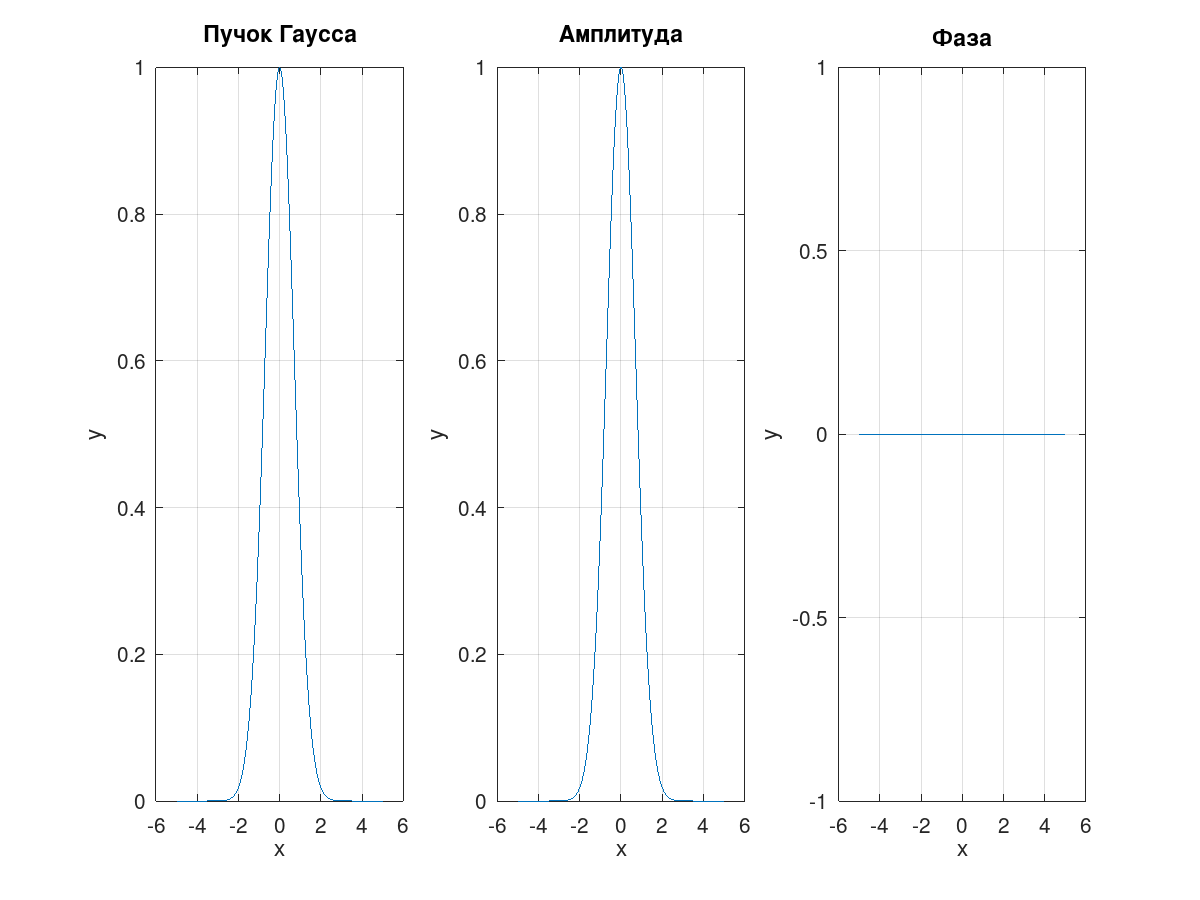
\includegraphics[width=0.75\pagewidth]{gauss}
				\caption{Графики гауссова пучка, амплитуды и фазы}
				\label{gauss}
			\end{figure}
		}
		
		\item{
			Проверка правильности реализации преобразования Фурье. На вход подается гауссов пучок, на выходе получаем другой гауссов пучок -- рисунок \ref{gauss_check}. Построены также графики амплитуды и фазы.
			
			\begin{figure}[H]
				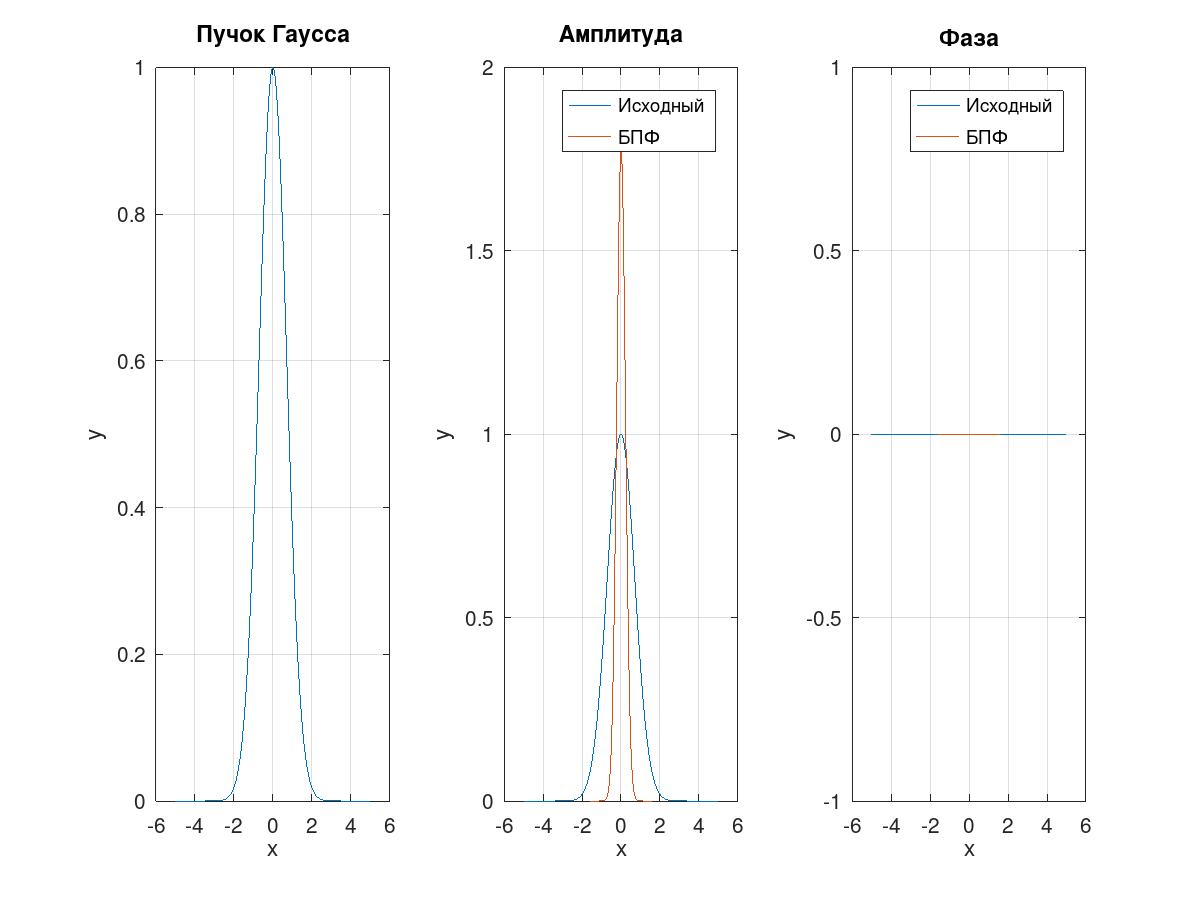
\includegraphics[width=0.75\pagewidth]{gauss_check}
				\caption{Графики гауссова пучка, амплитуды и фазы}
				\label{gauss_check}
			\end{figure}
		}
		
		\item{
		Реализуем финитное преобразование Фурье стандартным методом численного интегрирования -- методом прямоугольников \eqref{rect_method}.
		\begin{equation}\label{rect_method}
		\int\limits_a^b f(x) dx = \sum\limits_{k=1}^n f(\dfrac{x_{i - 1} + x_i}{2} (x_i - x_{i - 1}).
		\end{equation}
		
			Приведём реализацию метода численного интегрирования (полный код представлен в приложении А):
			
		\inputminted[breaklines, mathescape, fontsize=\footnotesize]{octave}{./src/num_integration.m}
		}
		
		\item{
		Сравнение преобразований Фурье: стандартным методом численного интегрирования и с помощью применения алгоритма БПФ. Результаты изображены на рисунке \ref{gauss_compare}.
		
			\begin{figure}[H]
				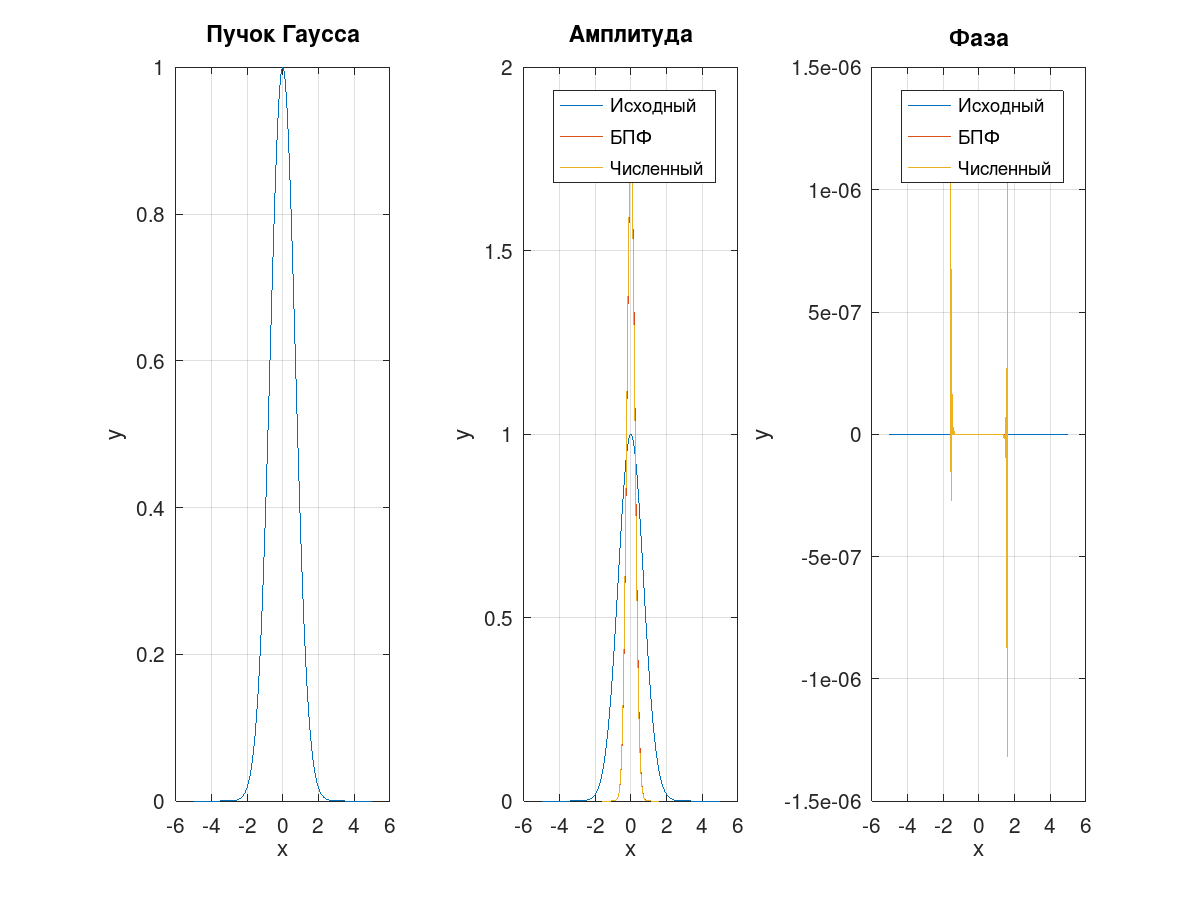
\includegraphics[width=0.75\pagewidth]{gauss_compare}
				\caption{Сравнение преобразований Фурье}
				\label{gauss_compare}
			\end{figure}
			
			Как видно из рисунка 3, численное преобразование Фурье, посчитанное с помощью метода прямоугольников совпадает с преобразованием Фурье, вычисленным с помощью алгоритма БПФ.
		}
		
		\item{
		На вход подается функция: $(4 x^2 - 2) e^{\frac{-x^2}{2}}$ , используется реализация преобразования Фурье через БПФ. Графики самого пучка и результат преобразования изображены на рисунке \ref{my_fft}.
		
			\begin{figure}[H]
				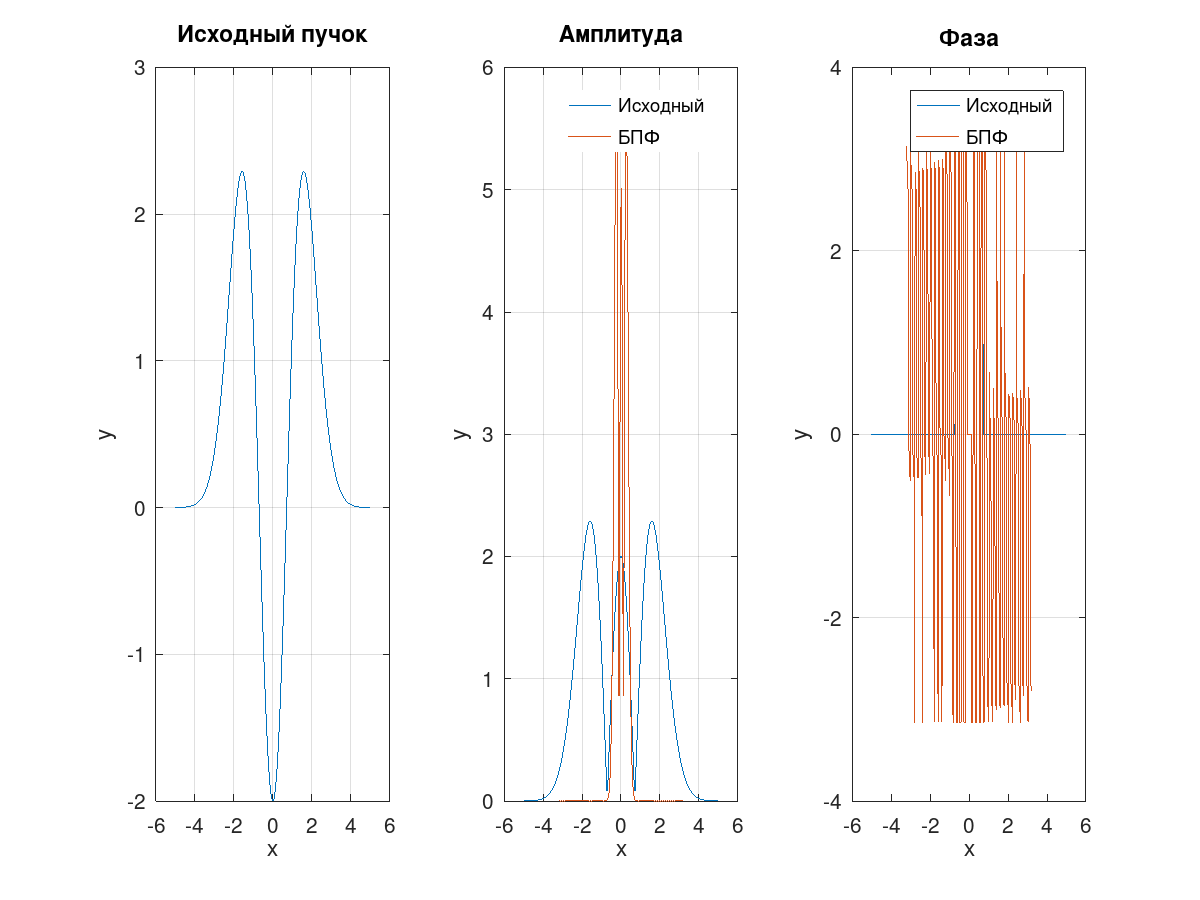
\includegraphics[width=0.75\pagewidth]{my_fft}
				\caption{Графики пучка, амплитуды и фазы}
				\label{my_fft}
			\end{figure}
		}
		
		\item{
			Найдём аналитическую форму для преобразования Фурье функции $(4 x^2 - 2) e^{\frac{-x^2}{2}}$.
			
			Сделаем замену $x = \sqrt{2} t$:
			\begin{equation}
			\int\limits_{-\infty}^{\infty} (4 x^2 - 2) e^{\frac{-x^2}{2}} e^{-2 \pi i x u} \,dx
			=  \sqrt{2} \int\limits_{-\infty}^{\infty} (8 t^2 - 2) e^{-t^2} e^{-2 \pi i t (u \sqrt{2})} \,dt. \nonumber
			\end{equation}
			
			Воспользуемся линейностью интегрирования:
			\begin{equation}\label{liniar}
			\sqrt{2} \int\limits_{-\infty}^{\infty} (8 t^2 - 2) e^{-t^2} e^{-2 \pi i t (u \sqrt{2})} \,dt
			= 2\sqrt{2} ( 4 \int\limits_{-\infty}^{\infty} t^2 e^{-t^2} e^{-2 \pi i t (u \sqrt{2})} \, dt - \int\limits_{-\infty}^{\infty} e^{-t^2} e^{-2 \pi i t (u \sqrt{2})} \, dt)
			\end{equation}
			
			Докажем следующие два соотношения:
			\begin{align}
			\label{et2}
			&\int\limits_{-\infty}^{\infty} e^{-t^2} e^{-2 \pi i t u} \, dt = \sqrt{\pi} e^{-\pi^2 u^2}, \\
			\label{deriv}
			&\int\limits_{-\infty}^{\infty} t f(t) e^{-2 \pi i t u} \, dt = -\frac{1}{2 \pi i} \frac{d F}{d u} (u).
			\end{align}
			
			Для доказательства \eqref{et2}, выделим полный квадрат:
			\begin{equation}
			\int\limits_{-\infty}^{\infty} e^{-t^2} e^{-2 \pi i t u} \, dt 
			= e^{-\pi^2 u^2} \int\limits_{-\infty}^{\infty} e^{-(t - \pi i u)^2} \, dt.\nonumber
			\end{equation}
			
			Сделаем замену $\xi = t - \pi i u$:
			\begin{equation}
			e^{-\pi^2 u^2} \int\limits_{-\infty}^{\infty} e^{-(t - \pi i u)^2} \, dt
			= e^{-\pi^2 u^2} \int\limits_{-\infty}^{\infty} e^{-\xi^2} \, d\xi.\nonumber
			\end{equation}
			
			Подставив интеграл Пуассона, получаем:
			\begin{equation}
			e^{-\pi^2 u^2} \int\limits_{-\infty}^{\infty} e^{-\xi^2} \, d\xi
			= \sqrt{\pi} e^{-\pi^2 u^2}.\nonumber
			\end{equation}
			
			Докажем \eqref{deriv}:
			\begin{equation*}
			\int\limits_{-\infty}^{\infty} \frac{d F}{d u} (u) e^{2 \pi i t u} \, du  = F(u) e^{2 \pi i u t} \vert_{u=\infty}^{\infty} - 2\pi i t \int\limits_{-\infty}^{\infty} F(u) e^{2 \pi i t u} \, du,
			\end{equation*}
			где первое слагаемое, в силу высокой осциляции, можно считать нулём. Таким образом получаем:
			\begin{equation*}
			\int\limits_{-\infty}^{\infty} \frac{d F}{d u} (u) e^{2 \pi i t u} \, du  = - 2\pi i t f(t).
			\end{equation*}
			
			Заметим что, из \eqref{deriv} следует \eqref{deriv2}:
			\begin{equation}\label{deriv2}
			\int\limits_{-\infty}^{\infty} t^2 f(t) e^{-2 \pi i t u} \, dt = \frac{1}{4 \pi^2} \frac{d^2 F}{d u^2} (u),
			\end{equation}
			
			Полсе подстановки \eqref{et2} и \eqref{deriv2} в \eqref{liniar} и упрощения, получаем:
			\begin{equation}
			\int\limits_{-\infty}^{\infty} (4 x^2 - 2) e^{\frac{-x^2}{2}} e^{-2 \pi i x u} \,dx
			= -2\sqrt{2 \pi} (8 \pi^2 u^2 - 1) e^{-2 pi^2 u^2}.\nonumber
			\end{equation}
			
			Результаты аналитического преобразования Фурье и преобразования Фурье через БПФ практически совпадают - рисунок \ref{full_solution}.
			\begin{figure}[H]
				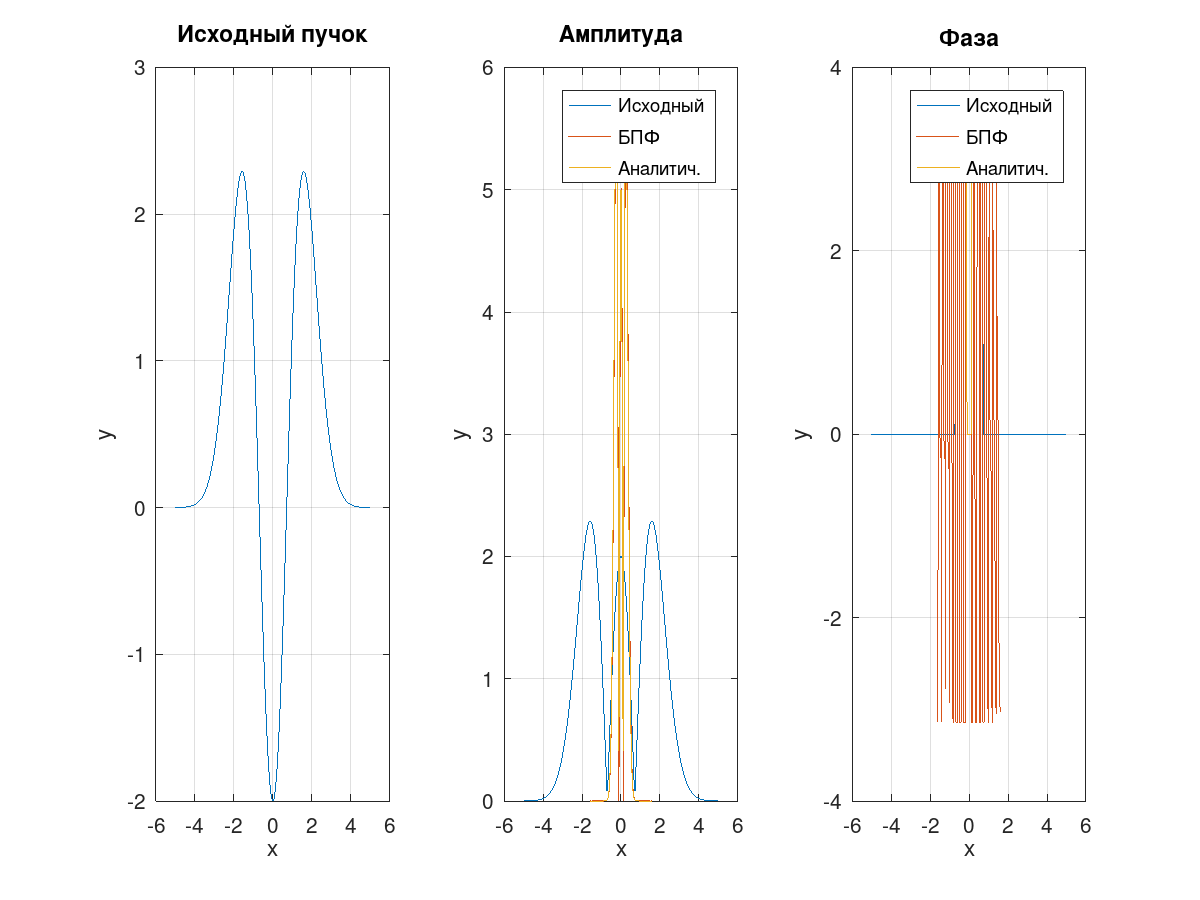
\includegraphics[width=0.75\pagewidth]{full_solution}
				\caption{Результаты аналитического решения и преобразования Фурье через БПФ}
				\label{full_solution}
			\end{figure}
		}
	\end{enumerate}
}
\newpage

\titleformat{\section}{\large\bfseries\centering}{\thesection}{0.5em}{\MakeUppercase}
\titleformat{\subsection}[block]{\bfseries\hspace{1em}}{\thesubsection}{0.5em}{}

\section*{Заключение}
{
	В данной лабораторной работе было реализовано одномерное финитное преобразование Фурье с помощью метода БПФ, а так же с помощью метода численного интегрирования. Был рассчитан теоритический результат преобразования Фурье для функции $(4 x^2 - 2) e^{\frac{-x^2}{2}}$. Построены графики для сравнения результатов различных преобразований. Было выяснено, что результаты аналитического преобразования Фурье и преобразования Фурье чеерз БПФ.
}
\newpage

%------------------------------------------------
% Приложения. Коды программ и.т.д.
%------------------------------------------------

\section*{Приложение А}
{
\addcontentsline{toc}{section}{Приложение А Код программы}
	\begin{center}
	\textbf{Код программы}
	\end{center}
	\inputminted[breaklines, mathescape, fontsize=\footnotesize]{octave}{./src/full.m}
}

\end{document}
